
\begin{chapter}{Force Field Development for Two-Body Systems: Principles and
Practices}
\label{ch:pointer}

\newcommand{\vmultipolecolor}{\ensuremath{\sum\limits_{\textcolor{mon}{tu}}\textcolor{mon}{Q_t^i}T_{tu}\textcolor{mon}{Q_u^j}}\xspace}

\begin{section}{Overview}
\begin{subsection}{What is \pointer?}

overview

\end{subsection}
\begin{subsection}{What parameters do we get from \pointer?}



\newcommand{\bij}{\textcolor{black}{B_{ij}}}
\newcommand{\bijr}{\bij r}
\newcommand{\vmultipolecolor}{\ensuremath{\sum\limits_{tu}\textcolor{mon}{Q_t^i}T_{tu}\textcolor{mon}{Q_u^j}}\xspace}
%% \begin{align}
%% \label{eq:pointer-ff_form}
%% \vdisp_{ij}
%% \intertext{where}
%% \begin{split}
%% \label{eq:ff_details}
%% \A &= \color{fit} A_iA_j \\
%% \B &= \sqrt{\textcolor{cfit}{B_iB_j}} \\
%% \C &= \sqrt{\textcolor{mon}{C_{i,2n}C_{j,2n}}} \\
%% P(\bij,r_{ij}) &= \frac13 (\bij r_{ij})^2 + \bij r_{ij} + 1 \\
%% f_{2n}(x) &= 1 - e^{-x} \sum \limits_{k=0}^{2n} \frac{(x)^k}{k!} \\
%% x &= \bijr_{ij} - \frac{2 \bij^2 r_{ij} + 3 \bij }
%% { \bij^2 r_{ij}^2 + 3 \bij r_{ij} + 3} r_{ij}
%% %\thinmuskip
%% \vrep_{ij} &= \textcolor{fit}{\Aex{ij}} P(\bij, r_{ij}) \exp(-\bijr_{ij}) \\
%% \velst_{ij} &= -\textcolor{fit}{\Ael{ij}} P(\bij, r_{ij}) \exp(-\bijr_{ij}) +
%% \vmultipolecolor
%% \\
%% \vind_{ij} &= -\textcolor{fit}{\Aind{ij}} P(\bij, r_{ij}) \exp(-\bijr_{ij}) + \textcolor{mon}{\vdrudeind} \\
%% \vdhf_{ij} &= -\textcolor{fit}{\Adhf{ij}} P(\bij, r_{ij}) \exp(-\bijr_{ij}) +
%% \textcolor{mon}{\vdrudescf} \\
%% \vdisp_{ij} &= -\textcolor{disp}{\Adisp{ij}} \sum\limits_{n=3}^{6} f_{2n}(x)
%% \frac{\textcolor{mon}{C_{ij,2n}}}{r_{ij}^{2n}} \\
%% %\thinmuskip
%% \vtot &= \sum\limits_{ij} \vrep_{ij} + \velst_{ij} + \vind_{ij} + \vdhf_{ij} +
%% \end{split}
%% \end{align}
%

\end{subsection}

========================================



What is \pointer

input and output parameters (as a workflow chart?)
    or as highlighted equation workflow

any important algorithmic details of the code

required input
    sapt file
    anisotropy file
    settings file
    (for advanced users) defaults file

tricky (i.e. not-yet-standardized) aspects of parameterization
    ccsdt correction
    electrostatics
        electrostatic damping (discuss how to change sapt file!)
        off-site point charges
    polarization damping - how to choose?
    exponents - when to fit vs. hold fixed?
    dispersion - when and how to fit (ccsdt correction vs sapt, how to choose
        asymptotic correction factor, caution in fitting)

documentation of various options and settings

wiki

Release version number

\end{section}

%% \begin{section}{A Philosophy for `Good' Two-Body Force Field Development}
%% \begin{enumerate}

\end{enumerate}


\begin{figure}
\centering
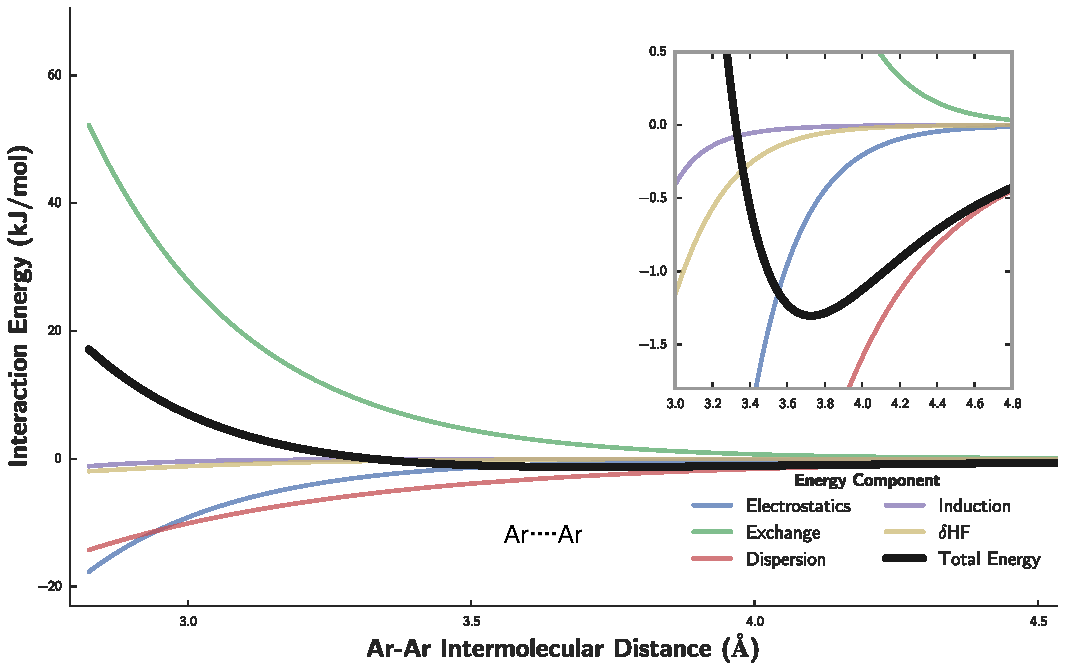
\includegraphics[width=\textwidth]{pointer/sapt.pdf}
\caption[\sapt-based force field fitting]
    {Fitting Force Fields with \sapt.
        }
\label{fig:pointer-sapt}
\end{figure}

%% \end{section}


\begin{section}{Parameterization Overview}
\begin{subsection}{Theory}

For \sapt-based force fields with functional forms similar to those in
\cref{ch:isaff,ch:mastiff} -- \mastiff being a prime example -- 
we have discussed in \cref{ch:workflow} a number of practical approaches for
intermolecular force field development.
(Here and throughout this Chapter, much of our
our discussion is restricted to examples with the \mastiff force field. Nevertheless, most
of the principles and ideas presented below should pertain generally to other
force fields (\saptff, \isaffold, etc.) that are fit on a term-by-term basis
to reproduce a benchmark \eda, and this Chapter is also intended to provide a
helpful guide for fitting and analyzing these types of force fields.)
In particular, we have already discussed strategies for optimally obtaining benchmark
electronic structure theory data and for calculating some of the parameters
that will be used in the final force fields themselves. Nevertheless, up
until now we have not focused on the actual process of force field fitting, nor on
strategies for assessing the quality of the resulting force fields. It is
to these two crucial topics that we now turn.

%%%%%%%%%%%% Fitting Equations %%%%%%%%%%%%%%%%%%%%%%%%%%%%%%%%%
\newcommand{\bij}{\textcolor{black}{B_{ij}}}
\newcommand{\bijr}{\bij r}
%\newcommand{\vmultipolecolor}{\ensuremath{\sum\limits_{\textcolor{mon}{tu}}\textcolor{mon}{Q_t^i}T_{tu}\textcolor{mon}{Q_u^j}}\xspace}

\begin{figure}
\begin{align}
%\label{eq:pointer-ff_form}
%\intertext{where}
\begin{split}
\label{eq:pointer-ff_form}
\A &= \color{fit} A_iA_j \\
\B &= \sqrt{\textcolor{cfit}{B_iB_j}} \\
\C &= \sqrt{\textcolor{mon}{C_{i,2n}C_{j,2n}}} \\
P(\bij,r_{ij}) &= \frac13 (\bij r_{ij})^2 + \bij r_{ij} + 1 \\
f_{2n}(x) &= 1 - e^{-x} \sum \limits_{k=0}^{2n} \frac{(x)^k}{k!} \\
x &= \bijr_{ij} - \frac{2 \bij^2 r_{ij} + 3 \bij }
{ \bij^2 r_{ij}^2 + 3 \bij r_{ij} + 3} r_{ij} \\[20pt]
%
\vrep_{ij} &= \textcolor{fit}{\Aex{ij}} P(\bij, r_{ij}) \exp(-\bijr_{ij}) \\
\velst_{ij} &= -\textcolor{fit}{\Ael{ij}} P(\bij, r_{ij}) \exp(-\bijr_{ij}) +
\vmultipolecolor
\\
\vind_{ij} &= -\textcolor{fit}{\Aind{ij}} P(\bij, r_{ij}) \exp(-\bijr_{ij}) + \textcolor{mon}{\vdrudeind} \\
\vdhf_{ij} &= -\textcolor{fit}{\Adhf{ij}} P(\bij, r_{ij}) \exp(-\bijr_{ij}) +
\textcolor{mon}{\vdrudescf} \\
\vdisp_{ij} &= -\textcolor{disp}{\Adisp{ij}} \sum\limits_{n=3}^{6} f_{2n}(x)
\frac{\textcolor{mon}{C_{ij,2n}}}{r_{ij}^{2n}} \\
\end{split}
\\[20pt]
\vtot &= \sum\limits_{ij} \vrep_{ij} + \velst_{ij} + \vind_{ij} + \vdhf_{ij} +
\vdisp_{ij}
\end{align}
\captionsetup{singlelinecheck=off}
\caption[Required parameters for \mastiff]
    {An overview of required force field parameters for the \mastiff and/or
\isaffold force fields. All relevant equations are
displayed in black, and the first instance of each parameter is shown in color according to the
following scheme:
\begin{itemize}
\item \textcolor{fit}{Unconstrained} parameters, which must be directly fit by \pointer
%
\item \textcolor{cfit}{Soft-constrained} parameters 
which, depending on user-specified settings, are treated as either soft- or
hard-constraints
%
\item \textcolor{mon}{Hard-Constrained} parameters read in by \pointer which are
always treated as hard constraints
\end{itemize}
See main text for details.
}
\label{fig:pointer-ff}
\end{figure}
%%%%%%%%%%%% Fitting Equations %%%%%%%%%%%%%%%%%%%%%%%%%%%%%%%%%


In regards to the force field fitting process, we begin by asking the obvious
question: "What parameters actually need to be fit in order to obtain a final
force field?" To this end, we have highlighted in \cref{fig:pointer-ff} all
of the parameters required to completely specify the \mastiff force field, and
have grouped these parameters according to how we choose to calculate/optimize
them in practice. In particular, all our force field parameters can be thought
of in terms of the following three categories:
%
\begin{itemize}
\item \textcolor{fit}{Unconstrained} parameters: These parameters have not
been specified on the basis of any monomer properties calculation, and so must
be directly fit to the two-body energy itself. 
%
\item \textcolor{cfit}{Soft-Constrained} parameters: These parameters
\emph{can} be fit entirely on the basis of monomer properties, however it is
sometimes advantageous to further refine this category of parameters with respect to the
benchmark two-body energies. In this case, soft
constraints\cite{Misquitta2016} are often applied to
the fitting process to ensure that the parameters do not deviate strongly from
their original values as calculated from monomer properties.
%
\item \textcolor{mon}{Hard-Constrained} parameters: These parameters are calculated
entirely from monomer properties, and are not futher involved in the force
field fitting process except as hard constraints.
\end{itemize}

To use \mastiff (see \cref{ch:mastiff}) as an example, an overview of the required parameters and
strategies for parameter fitting is as follows:
\begin{itemize}
\item \textcolor{fit}{\Aex{i}, \Ael{i}, \Aind{i}, \Adhf{i}}: 
The force field energy depends linearly on a number of short-range prefactors, and
in practice it is fairly straightforward to directly fit each of these
prefactors to the corresponding benchmark \sapt component energy. Note that, for anisotropic atomtypes,
each $A$ coefficient may in fact involve several parameters, all of which must
be directly fit:
\begin{align}
\label{eq:pointer-anisotropy}
\Aex{i}(\theta_i,\phi_i) &=
\textcolor{fit}{\Aex{i,\text{iso}}}\left(1 + 
\sum\limits_{l>0,k} \textcolor{fit}{\aex}  \mathcal{C}_{lk}(\theta_i,\phi_i)
\right)
\end{align}
(Though not entirely standard notation,\cite{stone2013theory}
for clarity in this Chapter we use
$\mathcal{C}$ to denote the set of renormalized spherical harmonics so as to
make a clear distinction between $\mathcal{C}$, the spherical harmonics, and
$C$, the dispersion coefficients from \cref{sec:workflow-dispersion}).
%
\item \textcolor{cfit}{$B_i$}:
The force field energy depends non-linearly on the short-range exponents \B,
making this parameter relatively difficult to optimize without constraints.
Fortunately, the \B parameters can
instead be calculated on the basis of monomer properties (see
\cref{sec:workflow-exponents}), and for obtaining force fields with
\rmse of \kjmol{\textasciitilde 1} it is often sufficient to use the \isa-obtained \B
parameters without further fitting. For obtaining more accurate force fields,
however, and in order to account for small uncertainties in our method of
obtaining \isa-derived \B parameters (see
\cref{sec:workflow-exponent_algorithm}), we have had good success in allowing the
\B parameter to vary slightly from its \isa-derived value. In practice, this entails
optimizing the \B parameters with respect to the benchmark \sapt exchange energy and subject
to a harmonic penalty function.\cite{Misquitta2016}
%
\item \textcolor{cfit}{\Adisp{i}}:
As with the other $A$ pre-factors, a pre-factor can be fit to the benchmark dispersion
energy so as to enhance the force field accuracy with respect to a given
benchmark electronic structure theory. (Vida infra, this benchmark energy can
either by \dftsapt or \ccsdt). Unlike with other pre-factors, however, and because we generally
have good accuracy in obtaining dispersion coefficients $C$ (see
\cref{sec:workflow-dispersion}),
nominally $\Adisp{i} \approx 1$ for most systems. Still, parameters must
sometimes be fit to the dispersion energy due to one or both of the following reasons: 
    \begin{enumerate}
    \item For anisotropic atoms, we must model the orientational dependence of
    the dispersion energy, and this model requires parameters outside of 
    the isotropic dispersion coefficients calculated in
    \cref{sec:workflow-dispersion}).
    \item Uncertainties in the \idma and/or \isa-pol dispersion coefficients can
    sometimes lead to inaccuracies in even the isotropic portion of the
    dispersion model, and these inaccuracies must sometimes be corrected by rescaling
    the isotropic dispersion coefficients themselves
    \end{enumerate}
In practice, when calculating \Adisp{ij} we often treat the \emph{anisotropic}
dispersion coefficients \adisp as free parameters, and sometimes additionally
optimize an \emph{isotropic} scale factor subject to
soft constraints.\footnotemark{ }
In total, this leads to the following set of parameters and equations for the
dispersion energy pre-factor:
%
\begin{align}
\Adisp{i}(\theta_i,\phi_i) &=
\textcolor{cfit}{\Adisp{i,\text{iso}}}
\left(1 + 
\sum\limits_{l>0,k} \textcolor{fit}{\adisp}  \mathcal{C}_{lk}(\theta_i,\phi_i)
\right)
\end{align}
where the colors serve to indicate that both free and soft-constrained
parameters may be contained within the pre-factor.
%
\item \textcolor{mon}{$Q^i_t$}:
Multipole moments $Q^i_t$ can be directly calculated from monomer properties
using the techniques discussed in \cref{sec:workflow-multipoles}. These
\isa-based multipoles are generally quite accurate, however (vida infra) when
using cheaper point charge models some care must be taken to ensure that the
effective model does not lead to a deterioration in force field accuracy 
%TODO: Reference where we discuss electrostatic models
\item \textcolor{mon}{\vdrude}:
As with multipole moments, polarization parameters
(\cref{sec:workflow-polarizabilities}) are treated as hard
constraints during the force field fitting process. Currently, there is not a
consensus on what functional forms and/or damping parameters should be used to 
model the short-range polarization energy, and this topic and its associated
practical issues will be the subject of \cref{sec:pointer-polarization}.
\item \textcolor{mon}{$C_{i,2n}$}:
Dispersion coefficients are calculated via the approaches discussed in
\cref{sec:workflow-dispersion}, and are generally treated as hard constraints in the
force field fitting process. In some cases (vida supra), these dispersion
coefficients are scaled to reproduce the \sapt energies, however we discuss in
\cref{sec:pointer-dispersion} some practical issues involved with such
scaling.
\end{itemize}


\footnotetext{
Currently, two constraints schemes are possible for 
$\Adisp{i,\text{iso}}$. First, we can treat this parameter as a hard
constraint, which sets $\Adisp{i,\text{iso}} = 1$. Second, we can apply
boundary conditions to treat $\Adisp{i,\text{iso}}$ as a free parameter
within the range $ 0.7 \le \Adisp{i,\text{iso}} \le 1.3 $. In future versions
of the \pointer code, we may also include the option of fitting
$\Adisp{i,\text{iso}}$ subject to a harmonic penalty function.
}

\end{subsection}

\end{section}

\begin{section}{The \pointer Code}
\label{sec:pointer-pointer}
Having identified the required parameters that completely specify \mastiff
and other similar force fields, we now turn to a discussion of the actual
fitting process itself. We begin in this section with an overview of the
software used to optimize each unconstrained/soft-constrained parameter, and
next (in \cref{sec:pointer-fitting}) discuss principles and practices
related to fitting each component of the benchmark \sapt energy.

As the name suggests, the \acrfull{pointer} is a Python package developed to aid in the fitting of
(two-body + $N$-body polarization) intermolecular force fields. \pointer is
open-source and is available for download from
\url{https://git.chem.wisc.edu/schmidt/force_fields}.
%TODO: Update this url and the one below for the pointer code once it's been
%uploaded to github
Documentation and examples for using \pointer are available through the wiki at
\url{https://git.chem.wisc.edu/schmidt/force_fields/wikis/home}, but for
convenience we include here a brief overview of the program input, output, usage, and
main capabilities:


\begin{subsection}{Input}
Owing to the large number of parameters that serve as hard constraints in
fitting the final \mastiff force field
(see \cref{fig:pointer-ff}), a number of input parameters files are required
in \pointer.
Fortunately, provided the user has already executed the scripts and steps
from
\cref{ch:workflow}, all required input scripts should have all been created
automatically and copied over to the force field fitting subdirectory
(\verb|ff_fitting|) from which the \pointer code is intended to be run.
Thus in practice, \pointer is designed to be run in combination with the
Workflow so as to minimize the amount of required manual input.

In total, the following input files are required by the \pointer program,
where the tag <monomer> indicates that a separate file is required for each
unique monomer being fit. Files highlighted in
\textcolor{codegreen}{teal} or \textcolor{codepurple}{red} indicates that the input file
sometimes or always require
manual modification before running \pointer, whereas files in black are
created automatically from the various scripts used in the Workflow, and
usually don't require further alteration.

\begin{itemize}
\item \textbf{<monomer1>\_<monomer2>.sapt}:
Summarizes the output \sapt energies for each dimer configuration from
\cref{sec:workflow-geometries}, and specifies the atomtype for each atom in
each monomer 
\item \textbf{<monomer>.disp}:
Contains dispersion parameters for each monomer
\item \textbf{<monomer>.drude}:
Contains drude oscillator charges for each monomer
\item \textbf{<monomer>.exp}:
Contains short-range exponents for each monomer
\item \textbf{<monomer>\_<multipole\_suffix>.mom}:
Contains multipole moments for each monomer
\item \textbf{\_\_init\_\_.py}:
Empty file required to keep Python's module structure happy
\item \textcolor{codegreen}{\textbf{<monomer>.constraints}:}
Constraints file, used to include hard-constraints for any \A parameters
for any previously-fit atomtypes. See \cref{sec:pointer-advanced_options} for
details and \cref{lst:pointer-constraints} for an example input file.
\item \textcolor{codegreen}{\textbf{<monomer>.axes}:}
Axes file, used to specify the local axes and included spherical harmonics for
any anisotropic atomtypes. See \cref{sec:pointer-fitting} for details and
\cref{lst:pointer-axes} for an example input file.
\item \textcolor{codegreen}{\textbf{defaults.py}:}
List of default settings for the \pointer program; these defaults rarely need
to be changed for routine force field development. 
See \cref{lst:pointer-defaults} for an example input file.
\item \textcolor{codepurple}{\textbf{settings.py}:}
List of modular settings for the \pointer program; many of these settings can
get changed in the course of routine force field development. See
\cref{sec:pointer-fitting} for details and \cref{lst:pointer-settings} for
an example input file.
\end{itemize}

\end{subsection}

\begin{subsection}{Usage and Output}

Once the required input files have been created/modified, running the \pointer
program is straightforward:
\begin{lstlisting}
./run_pointer.py
\end{lstlisting}

After a few minutes of runtime, \pointer will generate the following important output
files (file prefixes and suffixes may differ slightly depending on the choice
of input variables \verb|file_prefix| and \verb|file_suffix| from \verb|settings.py|):
\begin{itemize}
\item \textbf{coeffs.out}:
Output file containing fit parameters and error metrics
\item \textbf{exchange.dat}:
\sapt and force field exchange energies given in a two-column format with
ordering identical to the input .sapt file
\item \textbf{electrostatics.dat}:
\sapt and force field electrostatic energies
\item \textbf{multipoles.dat}:
\sapt electrostatic and force field multipolar energies
\item \textbf{induction.dat}:
\sapt and force field second-order induction energies
\item \textbf{dhf.dat}:
\sapt and force field \dhf energies
\item \textbf{edrudes.dat}:
polarization energies, \vdrudeind and \vdrudescf, given in two-column format
\item \textbf{dispersion.dat}:
\sapt and force field dispersion energies
\item \textbf{total\_energy.dat}:
\sapt and force field total energies
\end{itemize}

We now discuss specific details related to the fitting of each energy
component.

\end{subsection}


\end{section}

\begin{section}{Force Field Fitting: Principles and Practice}
\label{sec:pointer-fitting}
In conjunction with the \pointer software, we can finally turn to the
main topics of interest in this Chapter: how can we accurately and
systematically develop intermolecular force fields? As discussed earlier,
with \mastiff
some aspects of the force field development process remain an `art', and are thus
usually guided by chemical intuition, whereas increasingly more aspects of force field
fitting now can be carried out in a systematic and reasonably black-box manner. Here
we offer an in-depth analysis of the force field development process for
\mastiff and related force fields, paying
specific attention to addressing both the `artistic' and `scientific' choices
that must be made when developing models for new systems. 

\begin{figure}
\centering
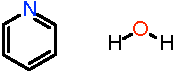
\includegraphics[width=0.3\textwidth]{pointer/molecules.pdf}
\caption{Pyridine and water -- molecular examples of challenges in force field fitting}
\label{fig:pointer-molecules}
\end{figure}

\begin{subsection}{General}

In general, a large number of development choices must be made prior to force field
fitting: which benchmark energies to use, how to sample the dimer \pes, which
parameters to treat as hard constraints, etc. While some of these choices have
been discussed in \cref{ch:workflow}, the following considerations also bear
mention:

\begin{paragraph}{Atom-typing}
In developing force fields for new systems (specifically with regards to the \mastiff approach, though
many of the principles below apply generally to other ab initio force fields),
an initial choice must be made as to how to categorize each atom into 
`atomtypes', where by definition all atoms within the same \atomtype share the
same force field functional form and parameters. In some cases, such as with
water, atomtyping is a fairly obvious decision, and it is easy to see how two
unique types should be used to describe the system. With other molecules
such as pyridine (\cref{fig:pointer-molecules}), however, this
atomtyping process is difficult to treat systematically and/or universally, and an iterative
guess-and-check process may be required to ascertain the number of atomtypes
that are required to obtain a desired level of force field accuracy (see
\cref{sec:pointer-exchange} for details).

Note that substantially increasing the number of free atomtypes (i.e., those
atomtypes whose parameters have not been pre-fit to a different system) 
can sometimes lead to numerical instabilities in fitting process or to
overfitting,\cite{Hawkins2004} and care must be taken with large/complex
systems to ensure good accuracy and transferability. 
\end{paragraph}

\begin{paragraph}{Anisotropy}
With the \mastiff approach, each atomtype can be treated as being either
isotropic or anisotropic, and for anisotropic atoms an arbitrary number of
spherical harmonic terms can be, in principle, included in the functional form. These spherical
harmonic expansions are always calculated with respect to a user-defined local
atomic coordinate system, and this coordinate system should be chosen so as to
maximize the symmetry (or approximate symmetry) of the system (vida infra).

For anisotropic atomtypes, in addition to specifying a local coordinate system
it is necessary to specify the ranks and orders of included spherical harmonic
functions $\mathcal{C}_{lk}$ that get included in
\cref{eq:pointer-anisotropy}. In practice, inclusion of spherical harmonics
beyond rank $l=2$ does not typically lead to worthwhile accuracy gains, and we
suggest truncation at this order for most systems.  Additionally, na\"ive
inclusion of all spherical harmonics up to rank 2 can lead to numerical
instabilities, and so only symmetry-allowed spherical harmonics (based on the
local coordinate system) should be included.  With the \pointer code, these
specifications for anisotropy are listed in the .axes file, with notation as
in \cref{lst:pointer-axes}. 

For most atomtypes (see \cref{ch:mastiff} for details), an isotropic description of the system is
sufficient, and so anisotropy should typically only be necessary for
atomtypes corresponding or spatially proximate to heteroatoms and/or multiple
bonding environments. Still, it is always worthwhile to explicitly test the effects of treating
different atoms anisotropically via comparison to the \sapt exchange energy
(see \cref{sec:pointer-exchange} for details). 

\end{paragraph}

\begin{paragraph}{Benchmark Energies and Correction Factors}

In \cref{ch:lmoeda}, we have discussed situations in which a
\sapt-based energy decomposition may be insufficient for force field
development, and have suggested strategies for improvement in these cases. 
For most systems, however, a \sapt-based decomposition will be of good
accuracy, and any deviations between \sapt and gold-standard \ccsdt can be accounted for using a \dccsdt correction
term as in \cref{ch:mastiff}.
Preliminary results on \co, \cl, \ho, and \nh suggest that this \dccsdt term
should be included as part of the dispersion energy (see \cref{sec:pointer-dispersion}), however
more systems should be tested to see if this practice is appropriate for
general force field development.
\end{paragraph}

\end{subsection}

\begin{subsection}{Exchange}
\label{sec:pointer-exchange}
From \cref{ch:isaff}, and as in \cref{eq:pointer-ff_form},
our exponentially-decaying model for the exchange-repulsion energy 
requires two sets of parameters per atomtype, \Aex{i} and $B_i$: 
%
\newcommand{\bij}{\textcolor{cfit}{B_{ij}}}
\newcommand{\bijr}{\bij r}
\begin{align}
\vrep_{ij} &= \textcolor{fit}{\Aex{ij}} P(\bij, r_{ij}) \exp(-\bijr_{ij})
\end{align}
%
Because the exchange-repulsion energy has no long-range contributions (unlike
with electrostatics, induction, and dispersion), when analyzing the final
force field it is often easiest to use the exchange energy (by itself) to
compare between models with differing numbers of atomtypes or treatments of
anisotropy. Additionally, when fitting the $B_i$ parameters against a harmonic
penalty function, \pointer takes advantage of the relative simplicity of the
exchange-repulsion model and fits this $B_i$ parameter based solely on the
exchange component.

\begin{paragraph}{Exponent Fitting}

To use \pointer to relax the $B_i$ parameters from their initial \isa-based values, the
following flag in \verb|settings.py| can be set to True:

\begin{lstlisting}[language=python]
...
# Exchange Settings: fit_bii selects whether or not to treat the ISA
# short-range exponents are soft- (fit_bii=True) or hard-constraints
# (fit_bii=False)
fit_bii                    =    True
...
\end{lstlisting}
In general, deviations from the input $B_i$ parameters should be no larger
than 5--10\%. Larger deviations may indicate problems with the calculated \bsisa
exponents or with the fitting process itself.

\end{paragraph}

\end{subsection}
\begin{subsection}{Electrostatics}
\label{sec:pointer-electrostatics}
Unlike with the exchange energy, the model for electrostatics must account for
both the effects of multipolar interactions (at long-range) and charge
penetration (at short-range):
%
\begin{align}
\velst_{ij} &= -\textcolor{fit}{\Ael{ij}} P(\B, r_{ij}) \exp(-\B r_{ij}) + \vmultipolecolor
\end{align}
%
\Ael{i} parameters are fit in a similar manner to the exchange energy, though
it is not recommended to attempt to re-fit the $B_i$ parameters to the
electrostatic energy. As for the multipole energy, in the simplest case (i.e.
without off-sites) these
parameters can simply be read in using the \verb|settings.py| file,
%
\begin{lstlisting}[language=python]
# Electrostatic Settings: choose which multipole files the program should use
multipoles_suffix          =   '_ISA-GRID_L2.mom'
\end{lstlisting}
%
where the \verb|multipoles_suffix| should point to some file
\verb|<monomer><multipoles_suffix>| in the \verb|input/| subdirectory.
In general, an $L2$ model is a good accuracy benchmark, and it's often useful
to compare the energies obtained from point-charge
models to those achievable with the $L2$ model.

\begin{paragraph}{Off-site models}
As described in \cref{ch:workflow}, practical software limitations and issues
of computational expense may sometimes require us to forego use of
higher-order multipole terms. 
When modeling the electrostatic energy via a point charge model, best accuracy
is often achieved by including off-site charges. Such off-site point charge
models can be treated using \pointer, though 
the following modifications to the standard input scripts are required:
\begin{enumerate}
\item Add the off-site positions to the .sapt file. Scripts for doing this are
discussed in \cref{sec:workflow-dimer_parameters}.
\item Modify the various monomer parameter files (located in the \verb|input/|
subdirectory to reflect the newly-added off-site positions:
    \begin{enumerate}
    \item Add dispersion coefficients (usually all zero) to each
            \verb|<monomer>.disp| file and for each atomtype
    \item Add extra blocks to each \verb|<monomer>.exp| corresponding to the
off-site positions. The .exp file(s) list exponents for each atom in the same
order as the .sapt file, and the .exp and .sapt file orderings must match.
Additionally, the off-site $B_i$ parameters must be set to a non-zero value to
avoid numerical errors.
    \item Add extra drude parameters to each off-site in the
\verb|<monomer>.drude| file. Atom ordering is as in the .sapt file, and
(assuming you do not want the off-sites to be polarizable) the drude charge
parameters should be set to zero.
    \item Assuming you do not wish short-range parameters to be fit to your
off-site atoms, add the names of all off-site atomtypes to \verb|defaults.py|:
\begin{lstlisting}[language=python]
lone_pair_flags                     =  ['Du' , 'lp']
\end{lstlisting}
    \end{enumerate}
\end{enumerate}
%
Energies between the off-site point charge model and the (more standard) $L2$/$L0$ models should
always be compared as a sanity check: if the errors in the offsite model are
larger than the errors from the $L0$ model, this is usually a sign that
something has gone wrong. On the other hand, if the electrostatic energies are
of a similar accuracy to those obtained with the $L2$ model, this indicates
that the point charge model is a fairly optimal description of the system's
multipolar electrostatics, and can be used without further modification in
molecular simulation.
\end{paragraph}


\end{subsection}
\begin{subsection}{Induction}
\label{sec:pointer-induction}
We turn now to a discussion of the \sapt induction energy, arguably the most
complicated energy component to understand and correctly model. Though there
is, as of yet, no one `best practice' for modeling the \sapt induction energy, a good
induction model will need to account for all of the following physical phenomenon:
\begin{itemize}
\item Long-range polarization
\item Polarization damping at short-range
\item Charge penetration effects arising from polarization
\item Charge transfer
\end{itemize}
Aside from long-range polarization, for which asymptotically-exact formulas
exist and can be modeled in simulation,\cite{Rick2002,Holt2008,Misquitta2007a,Misquitta2008b} 
there is currently little literature consensus as how best to separate out and
model the various physically-meaningful induction effects. Complicating matters further,
even though the \sapt induction energy is purely a 2-body effect, the
polarization model we develop based on the induction energy also implicitly defines
the model for \emph{many}-body polarization, which accounts for a sizeable
fraction of the total many-body energy discussed in
\cref{sec:pointer-many_body_effects}.
Consequently, it is easily possible to obtain an induction model which shows good
accuracy for dimer computations, but which leads to substantial inaccuracies
in modeling larger clusters or bulk liquids.

Improved induction models will certainly need to be the subject of future work,
and are discussed further in \cref{ch:conclusions}. In the meantime, below we present a summary of
common induction models that can be used to fit \sapt-based force fields.

\begin{paragraph}{Polarization}
For reasonably isotropic systems, long-range polarization effects can be described
either by a Drude oscillator model or via induced
dipoles.\cite{Rick2002,Lopes2009} In practice, these models tend to be
numerically similar, and we use them both during parameterization and
simulation.\footnotemark{} \pointer uses a Drude oscillator model for the
purposes of computing the polarization energy, and the Drude charges and
associated spring constants are read in as input in the \verb|<monomer>.drude|
file(s). These charges can be obtained using the methods described in
\cref{sec:workflow-polarizabilities}, however note that these charges are
sensitive to the choice of polarization damping model described below, and may
need to be refit if either the functional form or parameters for the damping
model are changed.

For more anisotropic systems (such as water), higher-order polarizabilities
have been shown to be important, and need to be included for best
accuracy.\cite{Cisneros2016,Misquitta2008b,Misquitta2016,Welch2008}
At present, however, higher-order polarizabilities have not been implemented
in most common software packages, and we are in the process of investigating
how to use off-site polarizabilities for modeling highly anisotropic systems.
\end{paragraph}

\footnotetext{In specific, Drude oscillator models have been used
historically in our group for their simplicity and ease of implementation.
More recently, we have begun running our simulations with the induced dipole
model in order to maintain compatibility with \openmm.}


\begin{paragraph}{Polarization Damping}
At short range, the induced dipole polarizabilities must be damped in order to
avoid the so-called `polarization catastrophe', an effect in which nearby
polarization sites mutually polarize each other to 
infinite values. While there is widespread consensus as to the importance and
necessity of including polarization damping, functional forms and parameters
for the polarization damping vary widely.\cite{Cieplak2009,Lopes2009,Thole1981,Slipchenko2009,Wang2011}
Thole-type damping functions\footnotemark{} are some of the more commonly used, and some
effort has been put forth to compare between several similar damping functions
and parameterization schemes.\cite{Wang2011,Wang2012,Liu2017}

Historically,\cite{McDaniel2013} several members of our group have used an
exponentially-decaying Thole function with an associated damping parameter of
2.0.\cite{Yu2011} More recently, and due to software limitations in \openmm,
we have taken to using the `Thole-tinker' model with a universal Thole damping
parameter $a=0.33$, which is reasonably similar to the damping parameter used by the
AMOEBA force field.\cite{VanVleet2017} Various Thole-type models can be
specified in \pointer
via the \verb|settings.py| file:
\begin{lstlisting}[language=python]
# Induction Settings: Choose the type and parameters for the polarization
# damping functions. Options for thole_damping_type are 'thole_tinker' and
# 'thole_exponential', and good defaults for thole_param are the 0.33 and 2.0 with
# respect to the two different damping types
# respectively
thole_damping_type         =   'thole_tinker'
thole_param                =    0.33
\end{lstlisting}
%
Note that the choice of Thole damping parameter can be very important, as this
modifies the relative balance between energies ascribed to polarization vs.
charge transfer, in turn modifying the magnitude of the many-body
polarization. In order to achieve a model that achieves the correct balance
between polarization and other inductive effects, future work may need to
involve some of the following advances:
\begin{enumerate}
\item Atomtype-specific Thole damping parameters
\item New functional forms for polarization damping
\item Explicit separation between the \sapt charge-transfer and polarization
energies. Several schemes have already been proposed to achieve this decomposition,
\cite{Bistoni2016,Misquitta2013,Horn2016b,Lao2016}
and the various available schemes should be tested for their utility in force field
development.
\end{enumerate}
\end{paragraph}

\footnotetext{Be advised, most papers in the literature will simply state that a
`Thole damping function' was used, but will not make explicit which of several
different Thole-type damping functions was meant.}

\begin{paragraph}{Charge transfer and inductive charge penetration}

In addition to polarization damping, charge transfer and inductive charge
penetration can become important at shorter intermolecular separations.
Physically-motivated functional forms for these effects are generally lacking,
though \citet{Misquitta2013} has suggested a double exponential decay,
and work in our own group has empirically found a single exponential decay
(with \isa-derived exponents $B_i$) to be reasonably satisfactory.

\end{paragraph}

\begin{paragraph}{Conclusions and Recommendations}

Our current approach to modeling inductive effects include a sum
over two contributions:
%
\begin{align}
\vind_{ij} &= -\textcolor{fit}{\Aind{ij}} P(\B, r_{ij}) \exp(-\B r_{ij}) + \textcolor{mon}{\vdrudeind} \\
\vdhf_{ij} &= -\textcolor{fit}{\Adhf{ij}} P(\B, r_{ij}) \exp(-\B r_{ij}) + \textcolor{mon}{\vdrudescf}
\end{align}
%
The \sapt benchmark separates the induction energy into 2\super{nd}- and higher-order
(i.e. \dhf) induction, and we fit both induction-like terms
separately.\footnotemark{} 
All parameters for the polarization model \vdrude are currently read in as hard
constraints, and the \Aind{i} and \Adhf{i} prefactors (which effectively accounts for both
charge transfer and charge penetration) are directly fit by \pointer.

\footnotetext{
Note that this expansion is in orders of perturbation theory,
not in orders of the \acrlong{mbe}.
}

\end{paragraph}


\end{subsection}
\begin{subsection}{Dispersion}
\label{sec:pointer-dispersion}
Dispersion is the last energy component that we must model in order to
completely describe the two-body energy. Asymptotically, the dispersion energy follows a
well-defined expansion in powers of $1/r^{2n}$, and at shorter distances the
energy expression is typically damped by a Tang-Toennies
function\cite{Tang1984,Tang1992} as follows:
%
\begin{align}
\vdisp_{ij} &= -{\Adisp{i}\Adisp{j}} \sum\limits_{n=3}^{6} f_{2n}(x)
\frac{\textcolor{mon}{C_{ij,2n}}}{r_{ij}^{2n}} \\
\Adisp{i}(\theta_i,\phi_i) &=
\textcolor{cfit}{\Adisp{i,\text{iso}}}
\left(1 +
\sum\limits_{l>0,k} \textcolor{fit}{\adisp}  \mathcal{C}_{lk}(\theta_i,\phi_i)
\right)
\end{align}
%
where $f(x)$ is the Tang-Toennies damping function from
\cref{eq:pointer-ff_form}, and the various colors highlight (as in
\cref{fig:pointer-ff}) the different ways in which the dispersion parameters
are calculated/fit.
Dispersion coefficients must always be read into
\pointer as input, and methods for obtaining these coefficients are as
described in  \cref{sec:workflow-dispersion}. 

In obtaining a final model for dispersion, it is important to ensure that any
model is quantitatively correct in the asymptotic regime, as the
least-squares optimization procedure \pointer uses does not ensure this
physically-correct behavior. Unless directly fitting atomtype-specific scale
factors to the dispersion energy (vida infra), a good strategy is to (using
the methods in \cref{sec:workflow-dispersion}) manually fit a universal scale factor to
the dispersion coefficients in order to achieve correct asymptotic behavior.
Once these scaled dispersion coefficients are read into \pointer, additional
anisotropic parameters can then be fit (or set to zero) by appropriate
modification of the \verb|settings.py| file:
\begin{lstlisting}[language=python]
# Dispersion Settings: Choose which parameters to fit to the dispersion
energies. Fit options
# include 'none' (to fit no parameters), 'anisotropic' (to just fit
# anisotropic dispersion parameters, but to leave isotropic dispersion
# coefficients unscaled), and 'all' (to fit both anisotropic and isotropic
# dispersion coefficients)
fit_dispersion             =    'anisotropic'
\end{lstlisting}

In select cases, such as when a \dccsdt correction is added to the
dispersion energy, it can be worthwhile to scale the isotropic
dispersion coefficients in an atomtype-specific manner. (This strategy was
used in \cref{ch:mastiff} to obtain dispersion parameters for \co, \nh, \ho,
and \cl.) This behavior is also allowed in \pointer using the above flags,
however care must be taken to ensure that this optimization does not degrade
accuracy in the asymptotic regime. In general, it is usually best to
\emph{not} fit isotropic scale factors to the dispersion energy in the absence
of significant improvements to the overall force field fit quality.


\end{subsection}
\begin{subsection}{Many-Body Effects}
As discussed above, some of the force field parameters that define the
two-body force field also contribute to the many-body energy. Polarization in
particular is inherently many-body, and (when possible) trimer energies should
be computed to ensure that the polarization model defined in
\cref{sec:pointer-induction} leads to good three-body energies.

For less polar systems, three-body dispersion and exchange can also be
important to include, and \citet{McDaniel2014} have shown how these
parameters can be directly calculated and modeled in the many-body
portion of the force field. This explicit three-body force field follows the
well-known Axilrod--Teller--Muto triple dipole functional form, and
\citen{McDaniel2014} describes how to obtain the necessary parameters. 

\end{subsection}
\end{section}

\begin{section}{Force Field Validation: Assessing Fit Quality}
\label{sec:pointer-validate}
Having obtained a final force field, the resulting model should always be
assessed and validated before use in molecular simulation. We divide this
topic into two sections -- sanity checks and validation -- to distinguish
between tests that can be performed via visual inspection of the fits compared
to those that require additional computations.

\begin{subsection}{Sanity Checks}

\begin{paragraph}{Visualization}

Once the \pointer code has been successfully run, the resulting force fields
should always be visualized, possibly with the aid of the included
visualization scripts,

\begin{lstlisting}
plot_compare_sapt_components.py -p <file_prefix> -s <file_suffix>'.dat' --display
plot_sapt_component_errors.py <file_prefix> <file_suffix>'.dat' --display
\end{lstlisting}

where additional visualization options are available by inserting the \verb|-h|
flag into the function call for either script. Such visualizations are shown,
using the pyridine dimer as an example, in
\cref{fig:pointer-pyridine_fits,fig:pointer-pyridine_errors}, and additional
visuals for water and other molecules are shown in
\cref{fig:pointer-water_fits,fig:pointer-water_errors,fig:pointer-asymptotic_water_fits,sec:mastiff-fits},
rspectively.

% \begin{landscape}
\begin{figure}
\centering
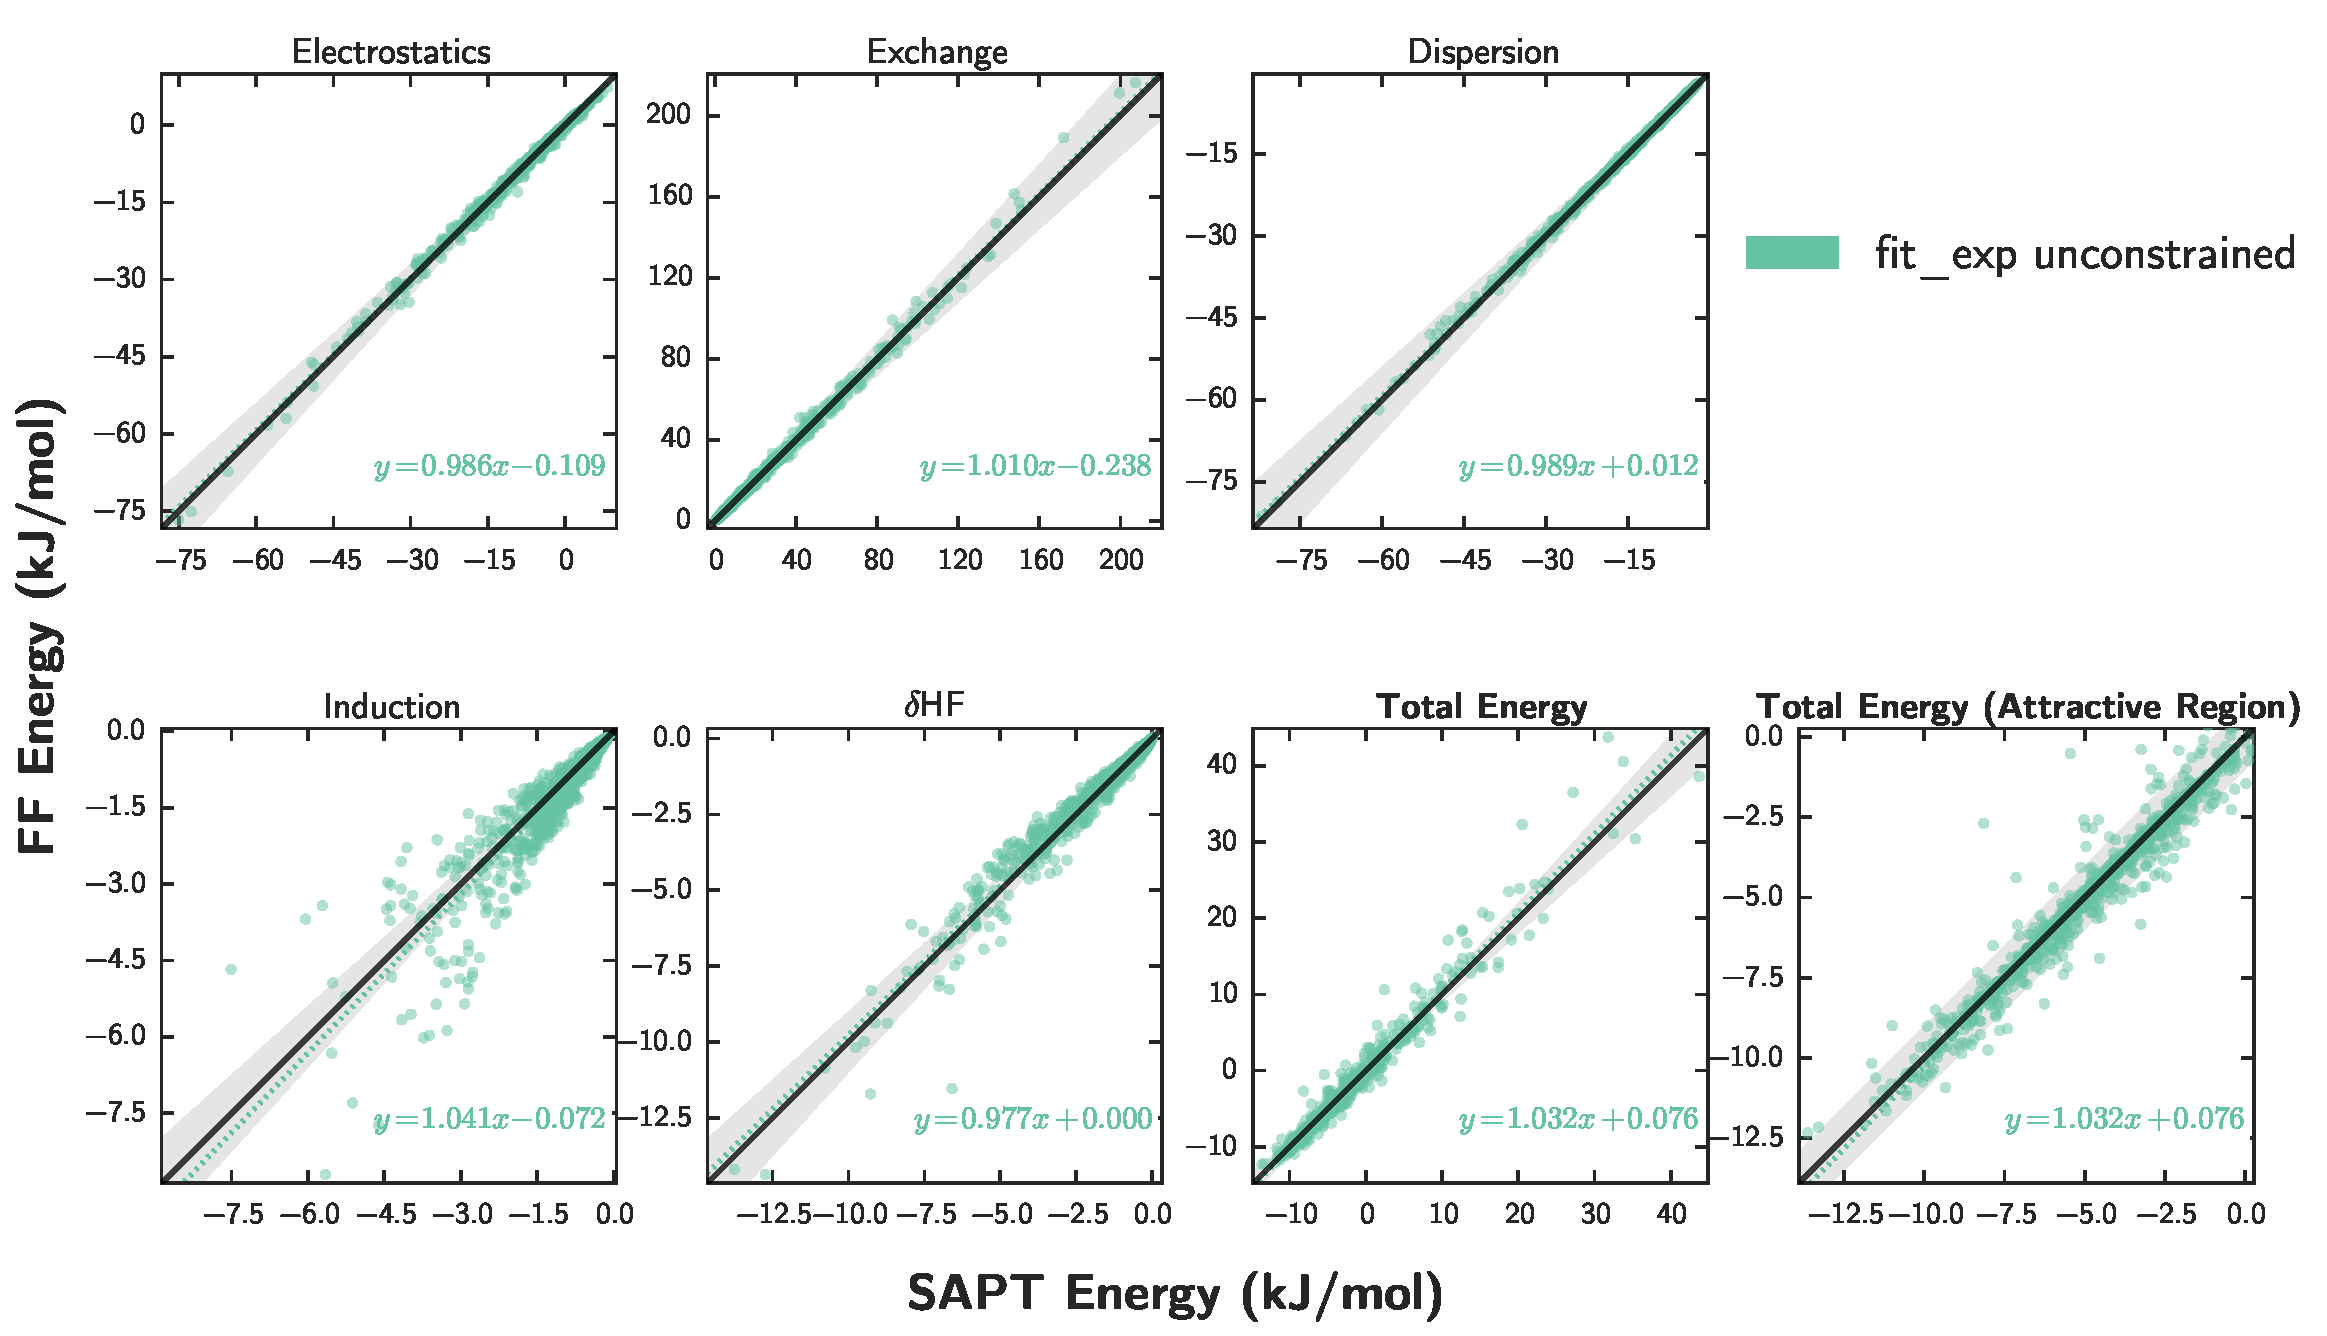
\includegraphics[width=\textwidth]{pointer/pyridine/sapt_comparison.pdf}
\caption[Comparison with the pyridine dimer]
{The pyridine dimer}
\label{fig:pointer-pyridine_fits}
\end{figure}

\begin{figure}
\centering
\fbox{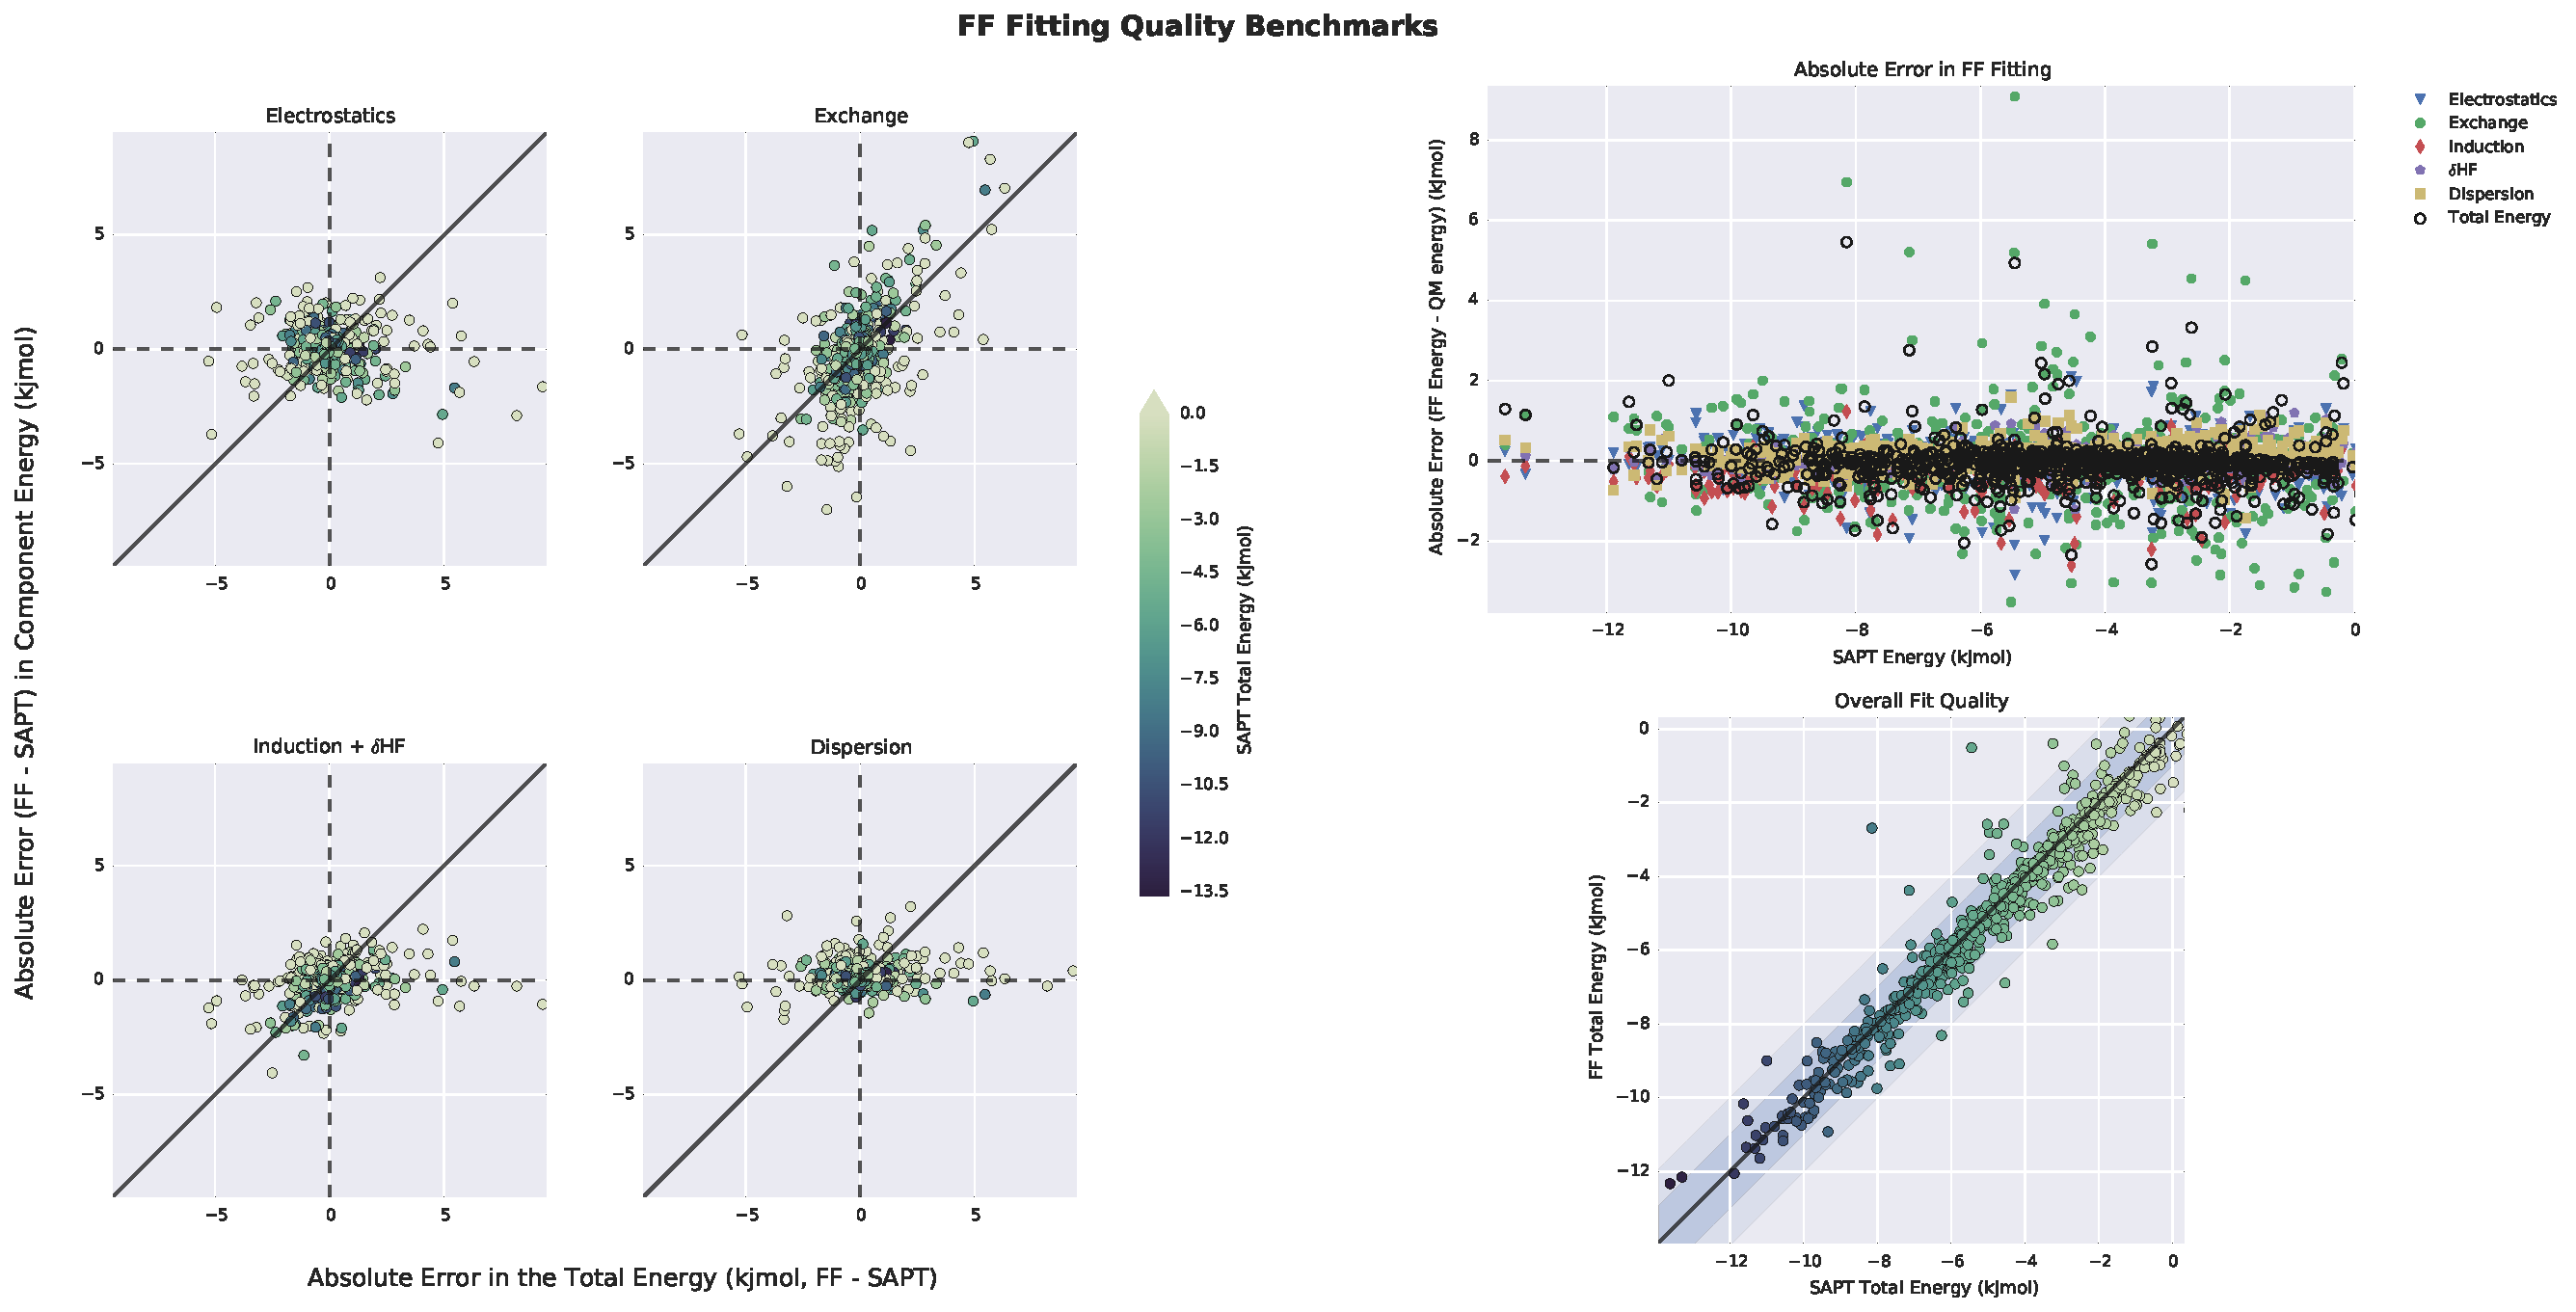
\includegraphics[width=\textwidth]{pointer/pyridine/fit_exp_sapt_errors.pdf}}
\caption[Errors with the pyridine dimer]
{The pyridine dimer errors}
\label{fig:pointer-pyridine_errors}
\end{figure}
% \end{landscape}

\begin{figure}
\centering
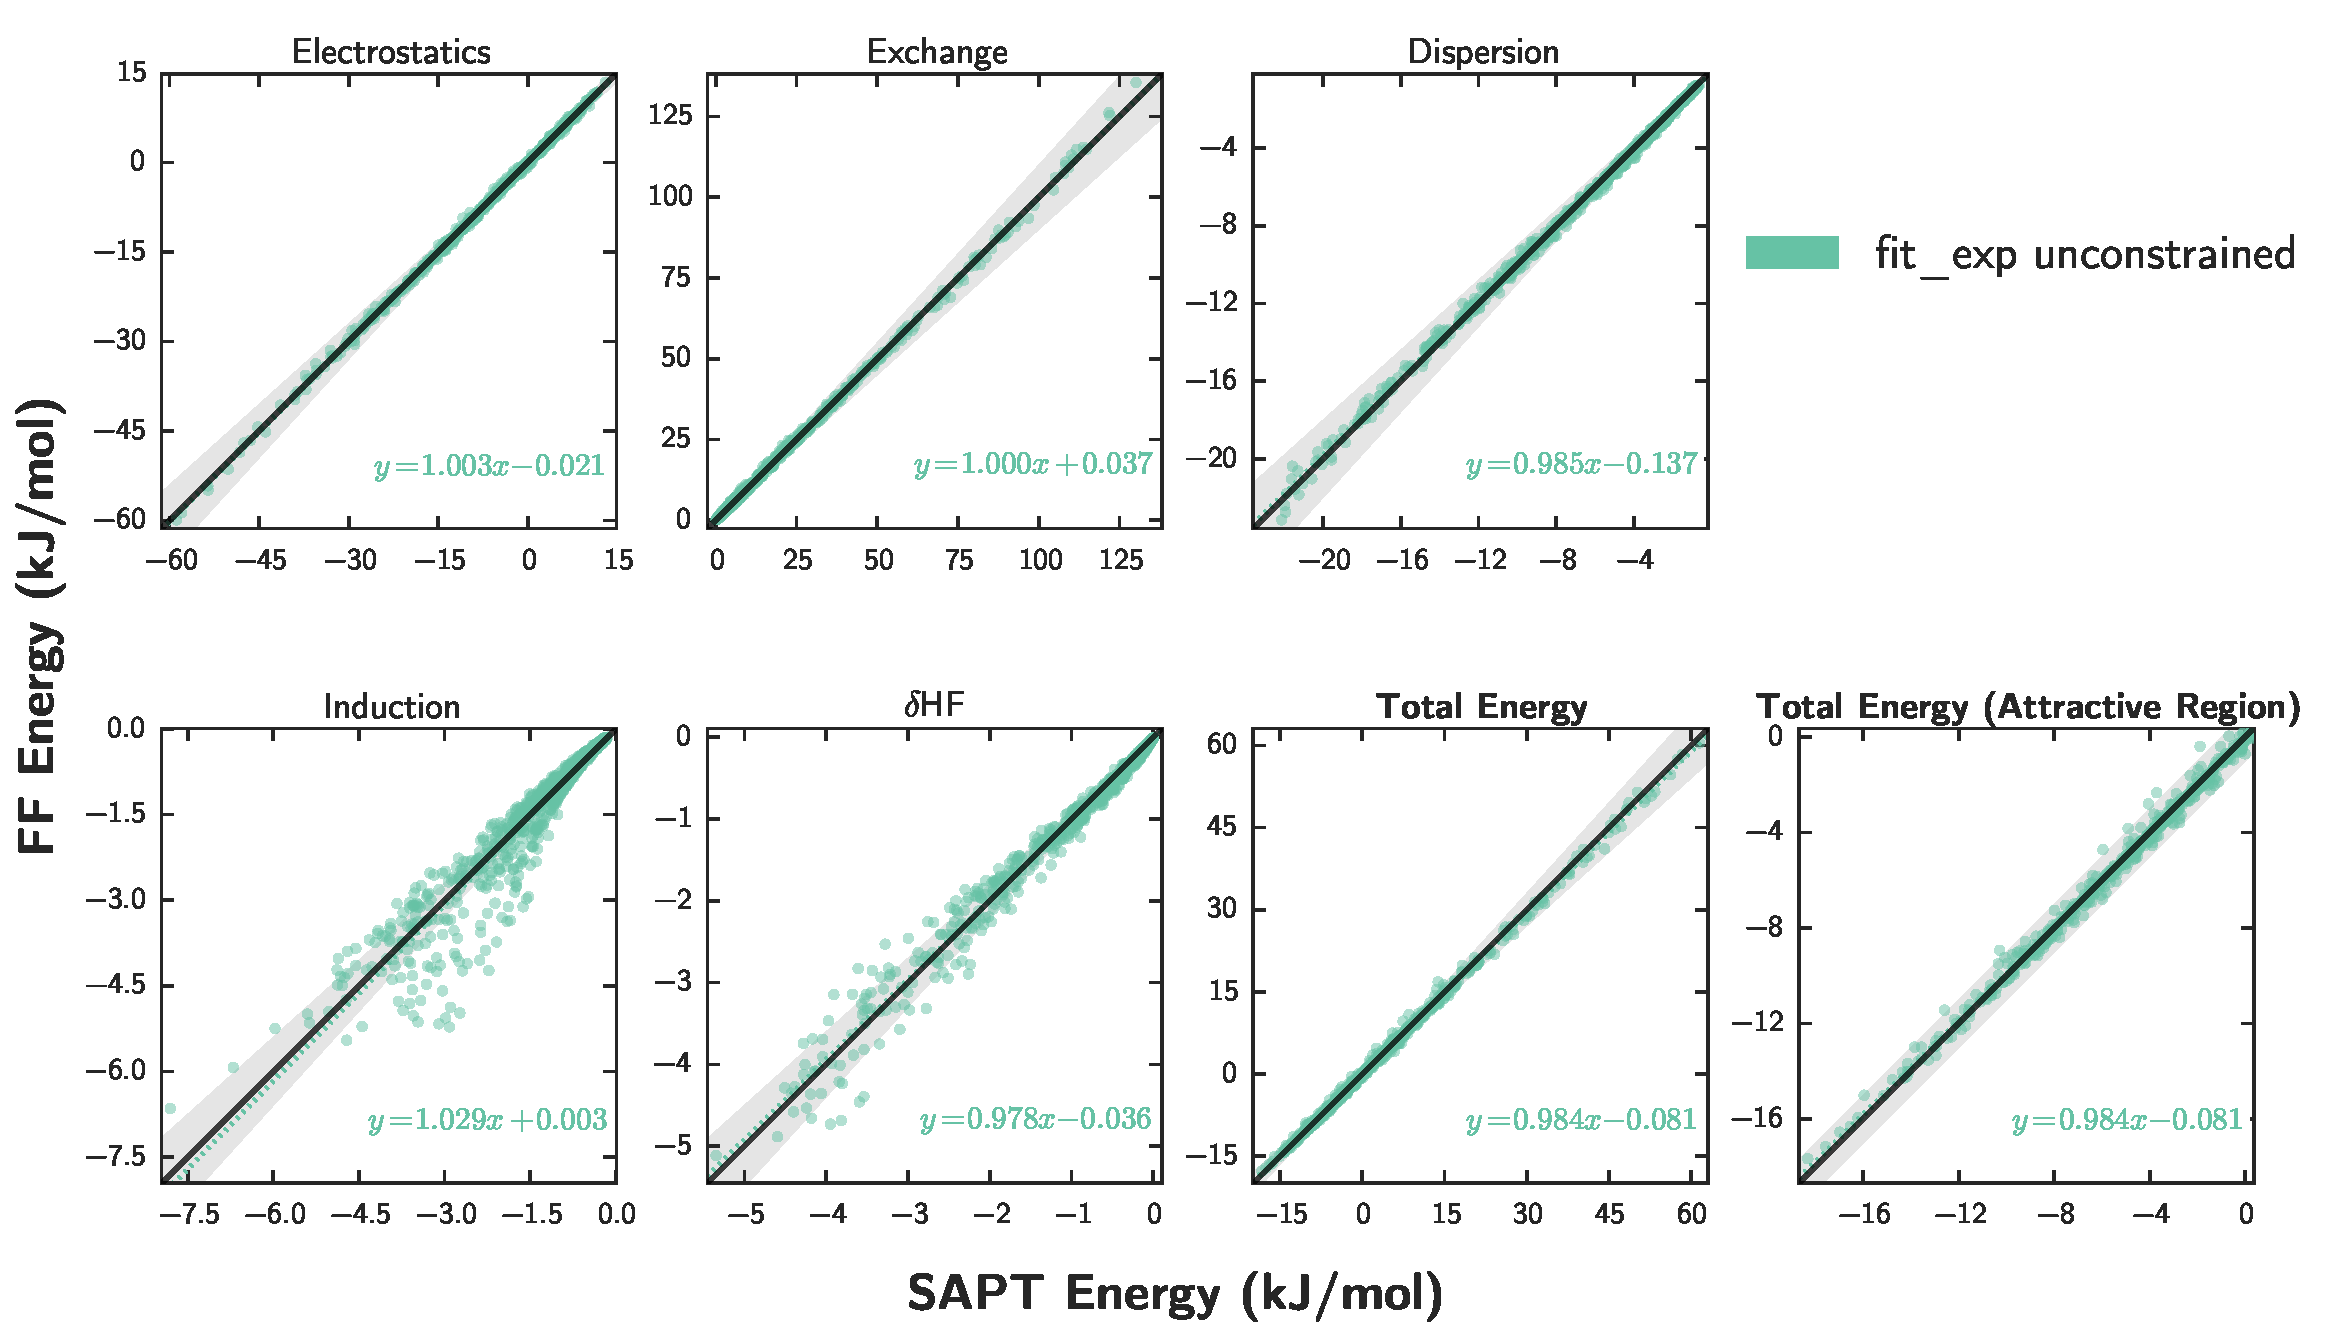
\includegraphics[width=\textwidth]{pointer/water/sapt_comparison.pdf}
\caption[Comparison with the water dimer]
{The water dimer}
\label{fig:pointer-water_fits}
\end{figure}


\begin{figure}
\centering
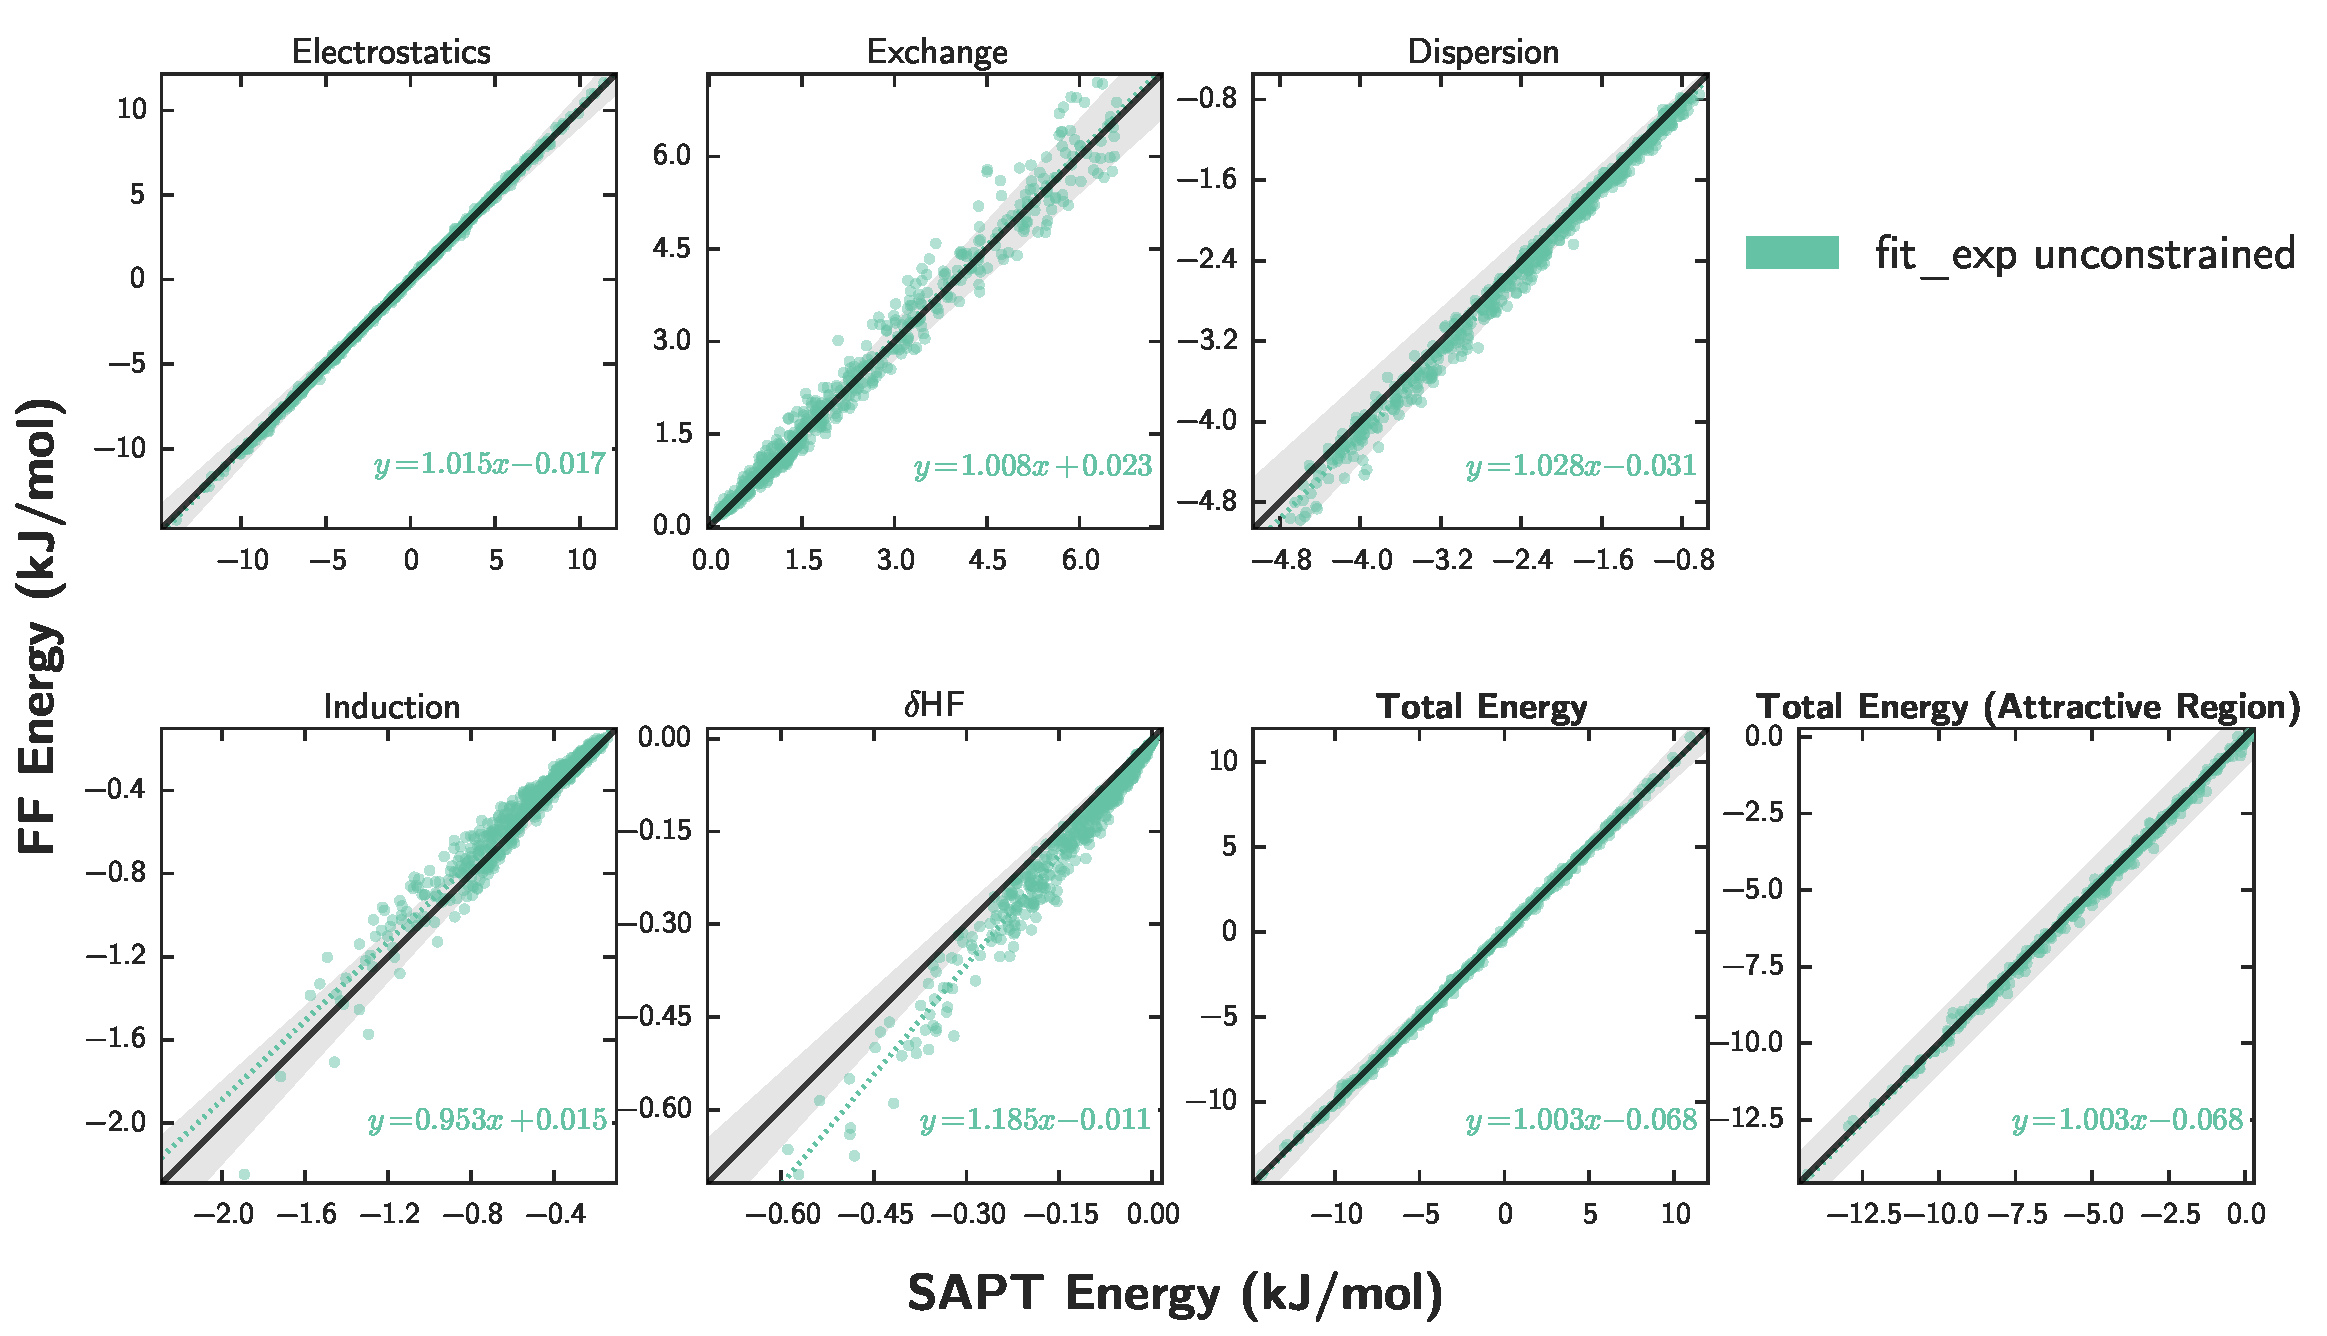
\includegraphics[width=\textwidth]{pointer/water/asymptotic_sapt_comparison.pdf}
\caption[Comparison with the water dimer]
{The water dimer}
\label{fig:pointer-asymptotic_water_fits}
\end{figure}

\begin{figure}
\centering
\fbox{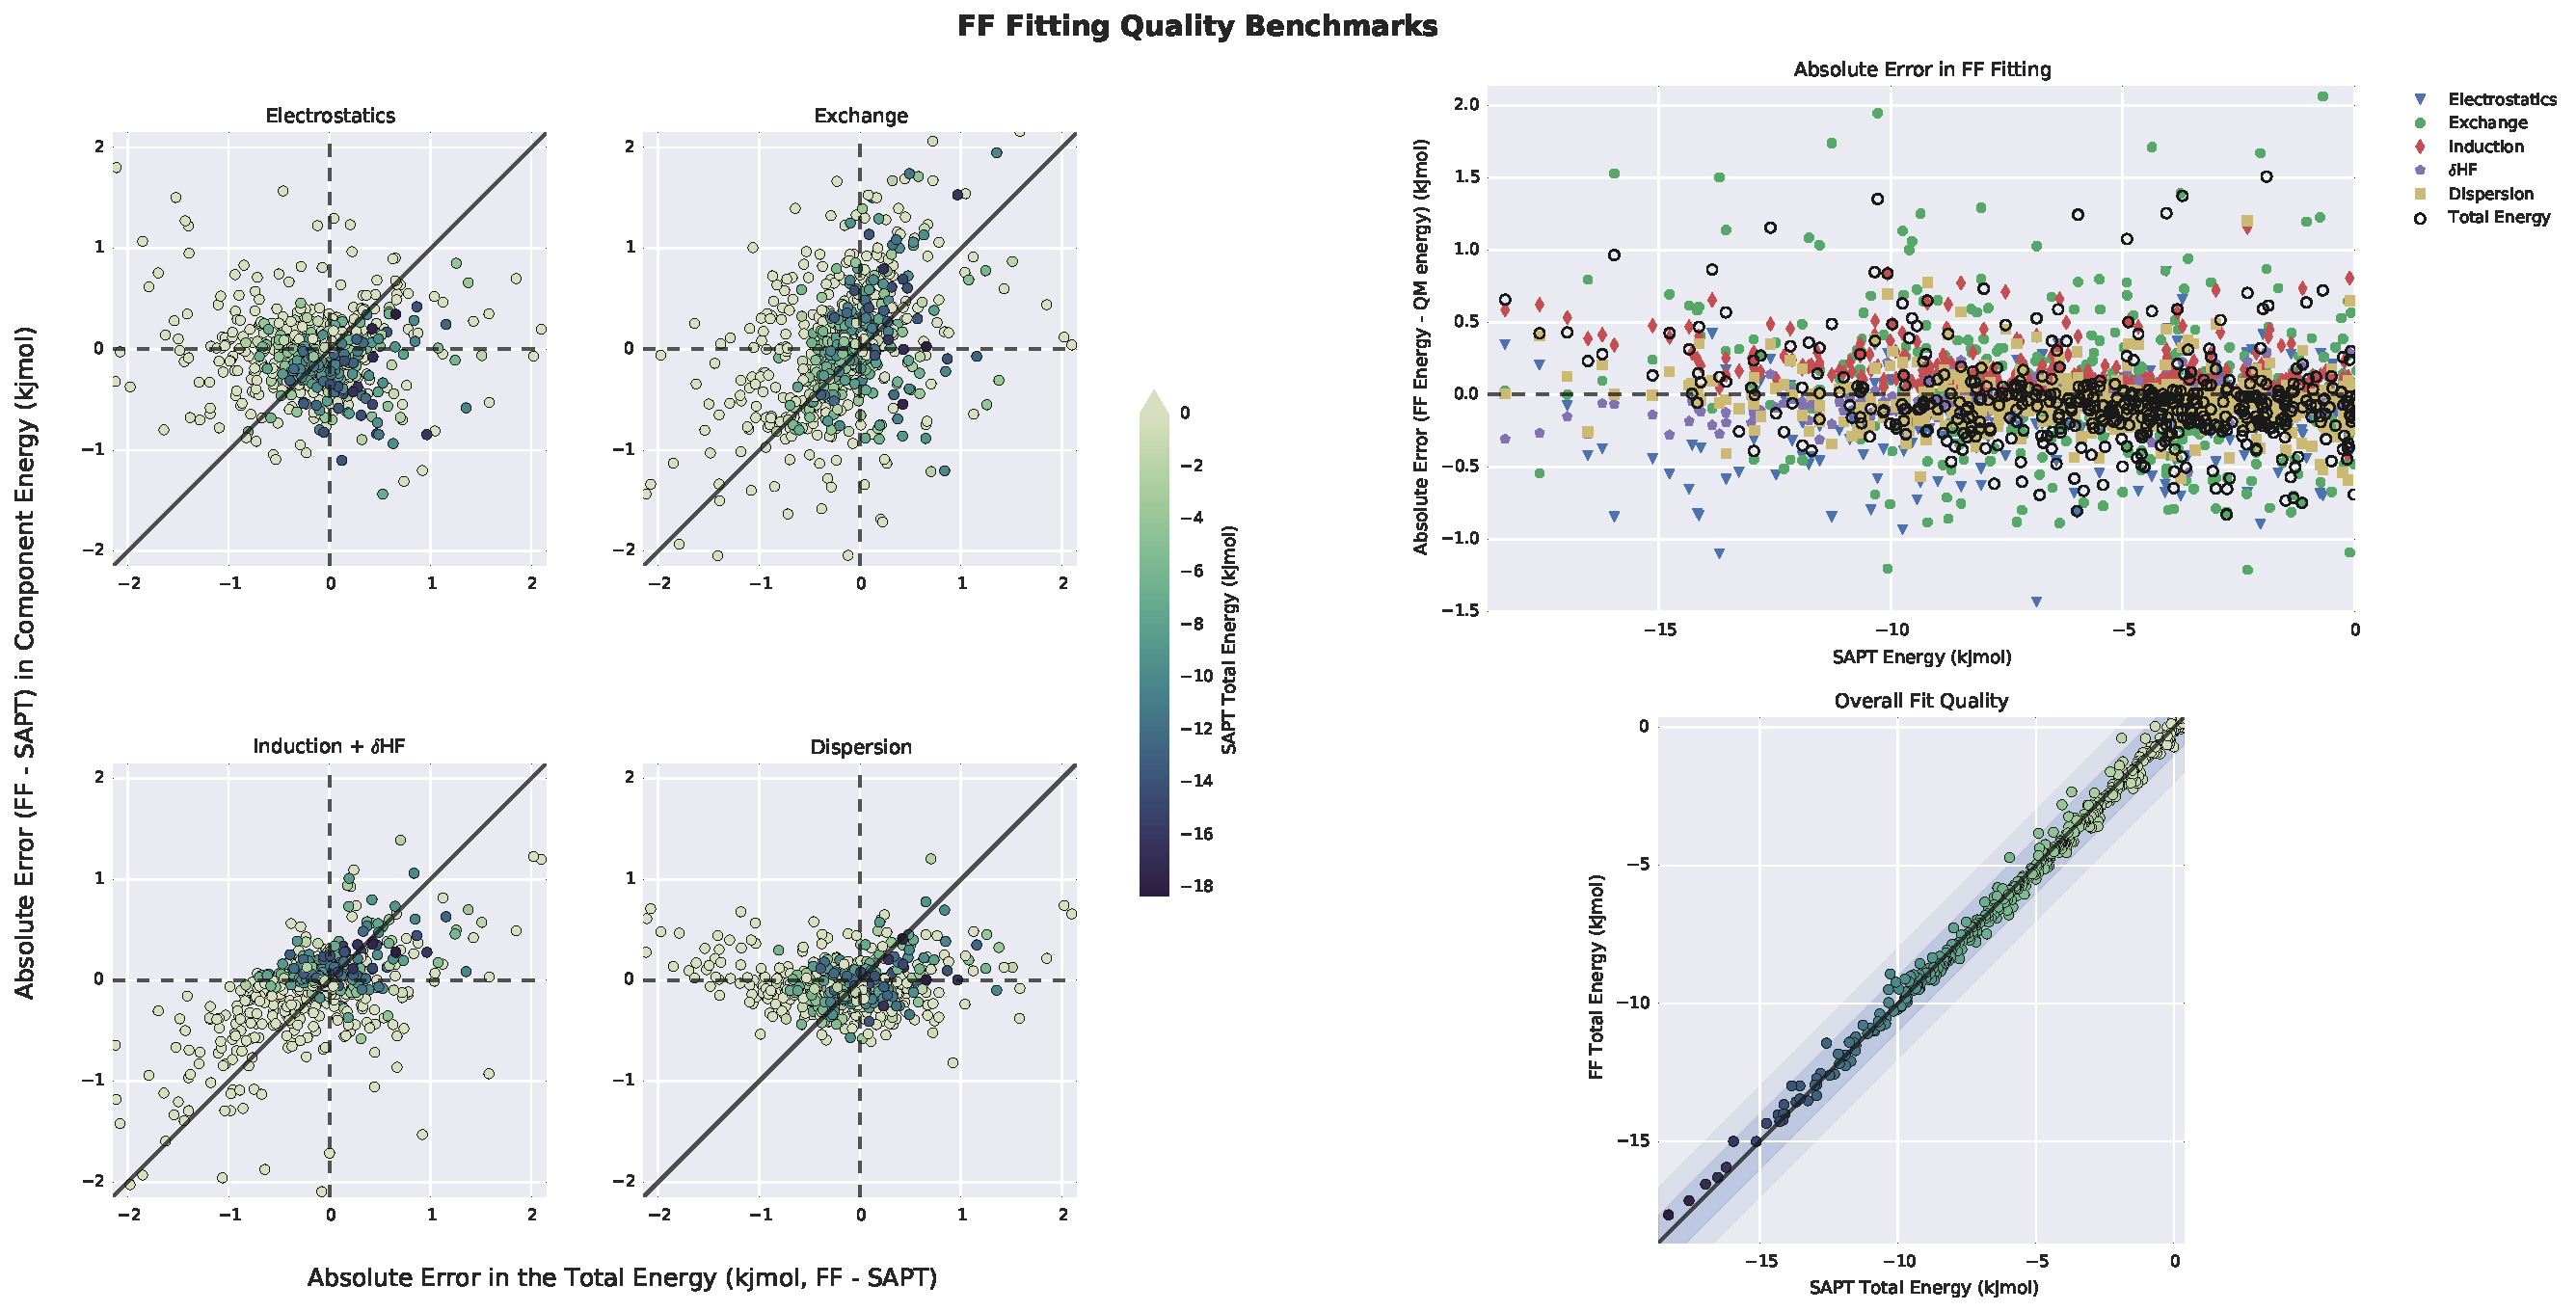
\includegraphics[width=\textwidth]{pointer/water/fit_exp_sapt_errors.pdf}}
\caption[Errors with the water dimer]
{The water dimer errors}
\label{fig:pointer-water_errors}
\end{figure}

\end{paragraph}


\begin{paragraph}{Error Analysis of the Minimum Energy Region}

As discussed in \cref{sec:workflow-geometries}, the mimimum energy region
plays a highly important role in simulations, and thus it is crucial that our
force fields correctly predict these energies. Ideally, the energy predictions
should be within \kjmol{$\pm 1$} of the benchmark energy, though larger errors
are easily possible when developing isotropic force fields. Even more
important than this precision, we must ensure that \emph{on average} the force
field energies are accurate in the minimum energy region. Any systematic
errors in the force field will have a pronounced effect on simulation quality,
particularly for studying bulk properties, as many properties depend only on
the average of system energy. 

\cref{fig:pointer-pyridine_errors,fig:pointer-water_errors} show errors in the minimum
energy region for both pyridine and water, and serve as illustrative examples.
These examples have been chosen because both force fields are relatively good quality, but also show errors that could
degrade simulation quality and be the focus of future improvement. 

In the case of pyridine, the force field fit shows fairly little systematic
error, and could probably be used to simulate bulk properties without issue.
Random errors on the order of \kjmol{0.5--1.0} are typical for this force
field, which may or may not be an issue depending on the desired accuracy
level and types of simulations one intends to run. 
(A few outliers show large errors compared to the
\sapt benchmark, however these points almost certainly reside along the
repulsive wall, judging by their exchange energies, and are thus not cause for
great concern.)
If one desired to improve
the precision of the pyridine force field, it is necessary to assess errors in
the force field on a component-by-component basis. \cref{fig:pointer-pyridine_errors}
shows how errors in the exchange component dominate the overall
error, and should be the first target for improvement. Since the exchange energy
only depends on a short-range exponential decay, this error could possibly be
mitigated by increasing the number of atomtypes (as shown, this force field
only has three atomtypes) or by including anisotropy on additional atomtypes,
as this potential only includes anisotropy on the nitrogen atom, and neglects
possibly-important anisotropies in the carbon atoms.

As for water, we see relatively little random error in the force field
(especially compared to the more isotropic models discussed in
\cref{ch:mastiff}), although again much of this random error can be attributed
to the exchange energy. In contrast to pyridine, however, we see some evidence
for systematic error in the water potential near the minimum energy
configurations. (Indeed, after testing our water force field against the
larger CC-pol database,\cite{Babin2013} we continued to find evidence for
overly-repulsive predictions in the minimum energy region.) This systematic
error, small as it may seem, is exacerbated in modeling larger clusters (vida
infra), and would need to be fixed before we could expect good success with
this force field in general simulations involving water. Looking at the errors on a
component-by-component basis, we can see that systematic errors in the potential
are heavily correlated with errors in the induction energy, making this
induction energy the most important target for improved modeling. As will be
discussed in \cref{ch:future}, improving our polarization model (both in terms
of the polarization damping and the long-range polarizabilities themselves)
will hopefully serve to reduce these systematic errors and improve the overall
quality of force fields for strongly polarizable molecules.

\end{paragraph}

\begin{paragraph}{Error Analysis of the Asymptotic Region}

In addition to the minimum energy region, it is important to ensure that the
asymptotic region of the potential is modeled correctly for each energy
component. This asymptotic analysis is shown for the water dimer in
\cref{fig:pointer-asymptotic_water_fits}, where we have shown force field fits
for each component, but have excluded configurations with exchange energies
above a certain threshold. (In general, the magnitude of the \sapt exchange
energy can be used as a proxy for the `short-rangeness' of a given
configuration.) 

Particularly for force fields that directly optimize the dispersion energy, it
is important to ensure that each energy component displays
asymptotically-correct behavior. This analysis can also be used to determine
optimal scaling values for the dispersion coefficients (see
\cref{sec:workflow-dispersion} for details).
\end{paragraph}


\end{subsection}
\begin{subsection}{Validation}

\begin{paragraph}{Trimer and Other Cluster Interaction Energies}

Currently, it is hard to guarantee that our polarization models will
correctly describe both the two- and three-body polarization energies. In
order to validate the many-body portion of the potential, trimer
interaction energies should be computed for a subset of energetically-important configurations
(preferably those taken from simulation) and compared to an accurate
electronic structure benchmark. These validation studies are especially
critical for highly-polar systems (such as water), as in these cases the
many-body polarization energy can account for a non-negligable fraction of the
total system energy. For such polar systems, it can also be important to study
the interactions of larger clusters in order to probe four-body and higher
interactions.\cite{Medders2015a,Cisneros2016,Medders2013}

\end{paragraph}

\begin{paragraph}{Simulations}

As the ultimate goal for many potentials is to be able to perform molecular
simulations, it is useful to validate new force field parameters in relation
to `simple' experimental properties. A reasonable starting point for such
comparisons is with the temperature-dependent 2\super{nd} virial coefficient, as this quantity is a
direct measure of the underlying two-body potential. Methods for calculating
the 2\super{nd} virial coefficient are discussed in \cref{ch:isaff,ch:mastiff}
and in \citens{Yu2011,McDaniel2013}.

In addition to the virial coefficient, a variety of other simulations form
useful comparisons to experiment (especially for studying bulk properties),
and examples of these can be found in 
\cref{ch:isaff,ch:mastiff} and in \citens{Yu2011,McDaniel2013,McDaniel2014}.

\end{paragraph}


\end{subsection}

\end{section}

\begin{section}{Summary and Outlook}
\label{sec:pointer-conclusions}
Throughout the past two Chapters, we have outlined a force field fitting
development methodology which enables an increasingly systematic
parameterization of intermolecular force fields.
By fitting these force field on a component-by-component basis, 
minimizing parameterization via frequent recourse to 
monomer properties calculations, and ensuring the physicality of the various
functional forms that get used in the final force field,
we now can reliably generate accurate and
transferable force field parameters for a broad class of materials and
molecular systems. Though invariably much work remains to be done in this
field, it is hoped that the principles and practices outlined in this Chapter
will sufficiently guide new force field developers in extending the
applications of the \mastiff methodology (or really, any \eda-based force
fields) to tackle new and interesting problems in molecular simulation.

\end{section}




\begin{subappendices}
\begin{section}{\pointer Input Files}
In total, \pointer requires modification of three input files,
as follows:

\clearpage
\lstinputlisting[language=python,
                 caption=settings.py,
                 label=lst:pointer-settings]{pointer/settings.py}

\clearpage
\lstinputlisting[language=python,
                 caption=defaults.py,
                 label=lst:pointer-defaults]{pointer/defaults.py}

\clearpage
\lstinputlisting[language=python,
                 caption={[pyridine.axes]
\textbf{pyridine.axes}.
For each anisotropic atomtype, the approximate symmetry and all terms included
in the spherical harmonic expansion are listed to the right of the atomtype.
Additionally, the local axis reference frame for each anisotropic atomtype is
defined in the Axes subsection using the z-then-x convention employed by
AMOEBA and other potentials (see \cref{ch:mastiff} for details). The first column of the axes subsection denotes
the index of the anisotropic atom (atom ordering as in the .sapt file), and the
second column denotes whether the z or x axis is being defined. For certain
local symmetries, the choice of x-axis is unimportant, and so not every
anisotropic atomtype has a defined x-axis. The remaining columns define the
direction vector for the axis in terms of atomic indices. The first index
(often the anisotropic atom itself) lists the start of the vector, and the
endpoint of the vector is defined as the midpoint of all subsequently listed
atoms.},
                 label=lst:pointer-axes]{pointer/pyridine.axes}

\clearpage
\lstinputlisting[language=python,
                 caption=pyridine.constraints,
                 label=lst:pointer-axes]{pointer/pyridine.constraints}

%% \scriptsize
%% \lstinputlisting[language=bash,
%%                  caption=dimer\_info.dat,
%%                  label=lst:workflow-dimer_info]{workflow/dimer_info.dat}
%% \normalsize
%% 
%% \scriptsize
%% \lstinputlisting[language=bash,
%%                  caption=pyridine\_pyridine.inp,
%%                  label=lst:workflow-dimer_geom]{workflow/pyridine_pyridine.inp}
%% \normalsize
%% 
%% \scriptsize
%% \lstinputlisting[language=bash,
%%                  caption=pyridine.atomtypes,
%%                  label=lst:workflow-pyridine.atomtypes]{workflow/pyridine_pyridine.inp}
%% \normalsize


\end{section}
\begin{section}{\pointer Output Files}
\clearpage
\lstinputlisting[   
                 %language=bash,
                 caption=coeffs.out,
                 label=lst:pointer-output]{pointer/coeffs.out}

\end{section}
\begin{section}{Additional Fitting Options}
\label{sec:pointer-advanced_options}
% Electrostatic damping types

% Slater charge penetration

% exact vs approximate slater functional form

% weighting temperature

% constrained A params

\end{section}
\end{subappendices}

\end{chapter}
